\documentclass{article}
\usepackage[utf8]{inputenc}
\usepackage{caption}
\usepackage[margin=1in]{geometry}
\usepackage{graphicx}
\graphicspath{ {Images/Assignment1/} }


\title{Assignment 1: GAM}
\author{Lorenzo Meninato}
\date{February 2018}

\begin{document}

\maketitle

Do women earn less than men at academic institutions? If so, what factors account for the differences in pay. 

\section{Introduction}
The Salaries dataset from the "car" package contains 2008-09 academic salary data for professors (assistant, associate, and full professors) for a single college in the US. Data was collected as part of the college's efforts to monitor salary differences between male and female professors. The dataset contains data on the salary, rank, discipline, sex, years of service, and years since PhD for 397 professors. In the following tables I give an overview of the summary statistics for the dataset. 
\begin{table}[ht]
\centering
\captionof{table}{Number of Observations by Rank and Sex} \label{t1} 
\begin{tabular}{rrrr}
  \hline
 & AsstProf & AssocProf & Prof \\ 
  \hline
Female &  11 &  10 &  18 \\ 
  Male &  56 &  54 & 248 \\ 
   \hline
\end{tabular}
\end{table}

There are a few concerns with the data. For starters, there is limited data on female professor salaries (only 39 observations). This could be difficult to work with, especially since the main problem we are trying to resolve is the difference in salaries between females and males, $\textit{ceteris paribus}$. Further, most professors are of the highest rank (266/397 observations), so if we group the sexes by rank and discipline, some group would have far too few observations\footnote{See Table 1.}. I also thought it would likely be that having both "Years since PhD" and "Years of Service" would be redundant and could lead to multicollinearity in later regressions\footnote{Especially when looking at linear models.}. Statistics confirm this later. 


At first glance, the subdivision of professors into applied and theoretical fields does not appear to be particularly useful, since it would likely be more fruitful to divide professors by what subject matter they teach, rather than if it is a theoretical or applied field. We would expect business professors to earn more than English professors, if outside market forces would pay the former more than the latter.

My analysis will primarily be Level 1 and Level 2. I think there will not be enough data to causally infer any relationships between variable, and further, I would not have the subject matter knowledge to adequately perform that type of causal inference. Therefore, any Level 3 analysis would be inappropriate. Still, I believe that from observing the summary statistics and univariate/bivariate statistics and plots (Level 1 analysis) I might be able to find appropriate models (or at least obtain useful information from the wrong models we might use) for the statistical relationships between variable (Level 2 analysis). While p-values and other forms of statistical inference are useful in many cases, descriptive analysis\footnote{In other words, a Level 1 regression analysis.} can still be quite useful in yielding useful insights about the data. Level 2 analysis, in the form of statistical tests and confidence intervals, while is certainly the most conventional form of statistics, can lead to very poor results without a solid justification for the methodology. Therefore, I must be careful about model and variable selection in both the ordinary linear models, and more complex generalized additive models (GAM).

\section{Univariate Analysis}

\begin{table}[ht]
\centering
\captionof{table}{Average Years of Service by Rank} \label{t2} 
\begin{tabular}{rlr}
  \hline
 & Rank & Years of Service \\ 
  \hline
 & AsstProf & 2.37 \\ 
  & AssocProf & 11.95 \\ 
   & Prof & 22.82 \\ 
   \hline
\end{tabular}
\end{table}

The results from Table \ref{t2} are not surprising. The higher the rank of the professor, the more years they have been working at the college. Table \ref{t3} might confirm the college administrators suspicions that female professors were underpaid relative to their male peers. At every rank, female professors have a lower median salary than their male colleagues. However, this difference might be accounted for in differences in experience ("Years since PhD") or discipline\footnote{Table 3 provides descriptive evidence of this, but certainly not indisputable proof.}.

\begin{table}[ht]
\centering
\captionof{table}{Median salaries by sex and rank} \label{t3} 

\begin{tabular}{rllr}
  \hline
 & Sex & Rank & Salary \\ 
  \hline
 & Female & AsstProf & 77000.00 \\ 
   & Male & AsstProf & 80182.00 \\ 
   & Female & AssocProf & 90556.50 \\ 
   & Male & AssocProf & 95626.50 \\ 
   & Female & Prof & 120257.50 \\ 
   & Male & Prof & 123996.00 \\ 
   \hline
\end{tabular}
\end{table}

\begin{table}[ht]
\centering
\captionof{table}{Average years since PhD by rank} \label{t4} 
\begin{tabular}{rlr}
  \hline
 & Rank & Years since PhD \\ 
  \hline
 & AsstProf & 5.10 \\ 
   & AssocProf & 15.45 \\ 
   & Prof & 28.30 \\ 
   \hline
\end{tabular}
\end{table}

Further, Table \ref{t5} suggests that applied disciplines tend to pay more than theoretical differences, by a median difference of about \$9000. When subdividing the disciplines by sex, the median salary for females in theoretical fields is nearly \$30000 less than in applied fields (\$8000 difference). But again, there is no reason to believe this is statistical evidence of gender pay discrimination. 

\begin{table}[!htb]
\centering
\captionof{table}{Median salary by sex and discipline} \label{t5} 
\begin{tabular}{rllr}
  \hline
 & Discipline & Sex & Salary \\ 
  \hline
 & A & Female & 78000.00 \\ 
   & B & Female & 105450.00 \\ 
   & A & Male & 105260.00 \\ 
   & B & Male & 113600.00 \\ 
   \hline
\end{tabular}
\end{table}

\newpage

The salary distribution is positively skewed. There seems to be certain clusters of salaries around certain price-points (\$75k, \$90k and \$105k). If there is a bias for administrators to pay amounts near certain round numbers, this could effect regression results later. An ordinary least squares approach would likely smooth out across the price-points, even if data points are clustered at those points, but perhaps in the GAM approach, if the B-splines are sufficiently sensitive we could expect there to be concave curves around those points. 

The "Years since PhD" data is a lot less right skewed than the years of service data. This could have been caused by the college hiring professors with prior experience. We would expect one of the primary determinants of college professor salary to be years of experience, as is common in most fields. Thus "Years since PhD" makes for a richer comparison between professors, since we could imagine that a professor with 20 years of experience would be paid more than a freshly minted PhD assistant professor. Given the difference in the skewness across those distributions, it might be that in the past 10 years the college has hired many professors, and not just recent PhDs. So perhaps any structural differences in pay by sex (across rank and discipline) might be due to inefficient contract negotiation of either new hires or established hires who have failed to renegotiate salaries effectively\footnote{Effective negotiation, in this context, would imply that professors are being paid close to the salary they could feasibly obtain at a similar institution.}

\begin{figure}[!htb]
    \centering
    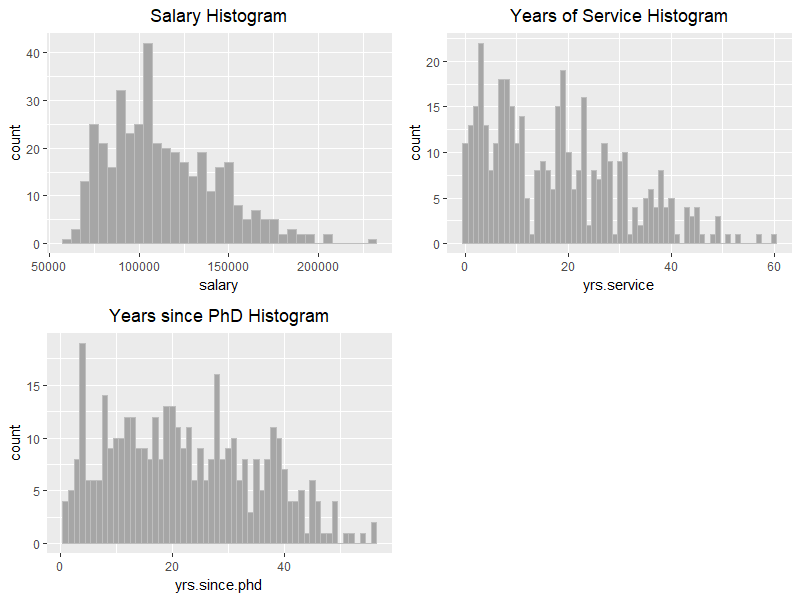
\includegraphics[scale=0.75]{Hist1}
    \caption{Histograms of Various Variables}
    \label{hist}
\end{figure}

\newpage

\section{Bivariate Analysis}

Histograms of "Years since PhD" and "Years of Service" visually suggest that the two variables are highly correlated. I think that it would be preferable to exclude "Years of Service" in a future report, since professors that have been researchers for many years at other schools would have less years of service, but likely could demand high salaries, since they have done much work since their PhD. 

Further, especially at the tail-end of these distributions, we can see that there is much less data for females beyond 25-30 years of experience. 
The histogram for female professors (for "Years since PhD"), is also nearly uniformly distributed, which we would not expect. These figures also demonstrate that for greater levels of work experience, e.g. $>20$ years of work experience, there is much less data for female professors. In terms of modelling, the results for more years of experience will likely be much noisier and less relevant for addressing the central concern of salary differences between sexes.

\begin{figure}[!htb]
    \centering
    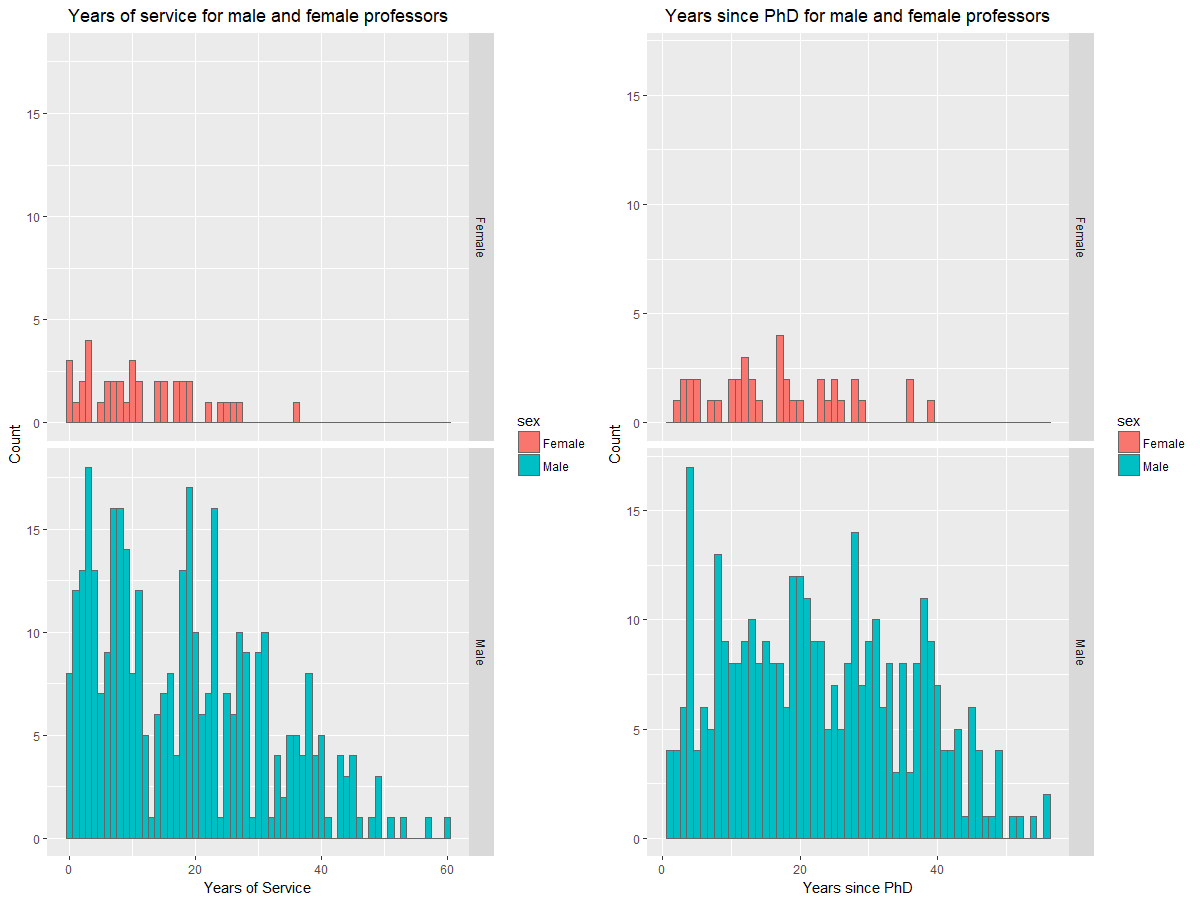
\includegraphics[scale=0.5]{YrsSex}
    \caption{Work Experience versus Sex}
    \label{pairs1}
\end{figure}

For females there is little data between \$75k and \$100k, with salaries tending to be clustered around those two boundaries. There could be a reason for this bimodal distribution. We do not know why this is the case. This could likely be explained by random variation in the data, and in particular, we would expect more noisy data since the data on female professors is so sparse.

\newpage

\begin{figure}[!htb]
    \centering
    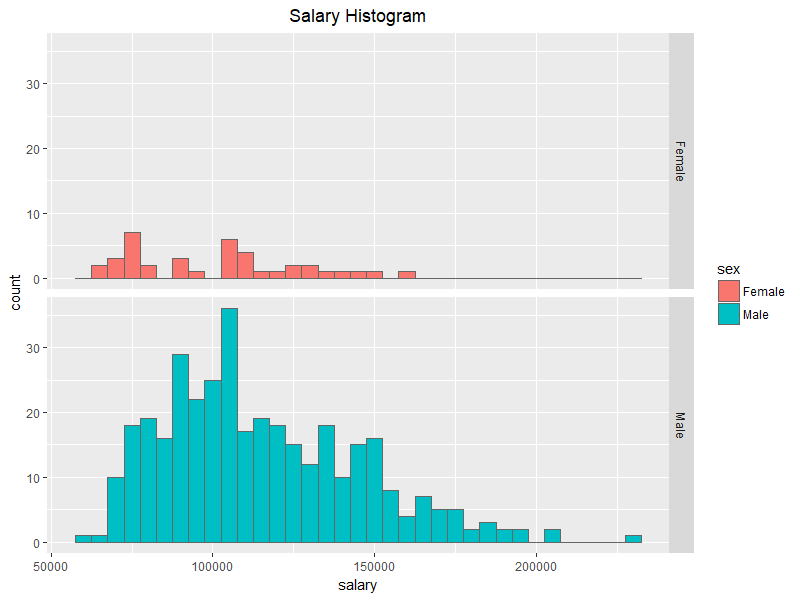
\includegraphics[scale=0.5]{salarySex}
    \caption{Salary versus Sex}
    \label{pairs2}
\end{figure}

For the violin plot\footnote{Violin plots are my preferred form of boxplots. They display similar information about a set of data, but they also describe how the data is distributed, which is useful for descriptive statistics like these.}, Figure \ref{pairs3}, note how the distribution of salaries is skewed right for assistant professors and full professors while it is skewed left for associate professors. This might be explained by the fact that assistant professors are more readily promoted to associate professor, and thus earn more, while associate professors might increase their salary over a longer period of time but would not be so easily promoted to full professor.


\begin{figure}[!htb]
    \centering
    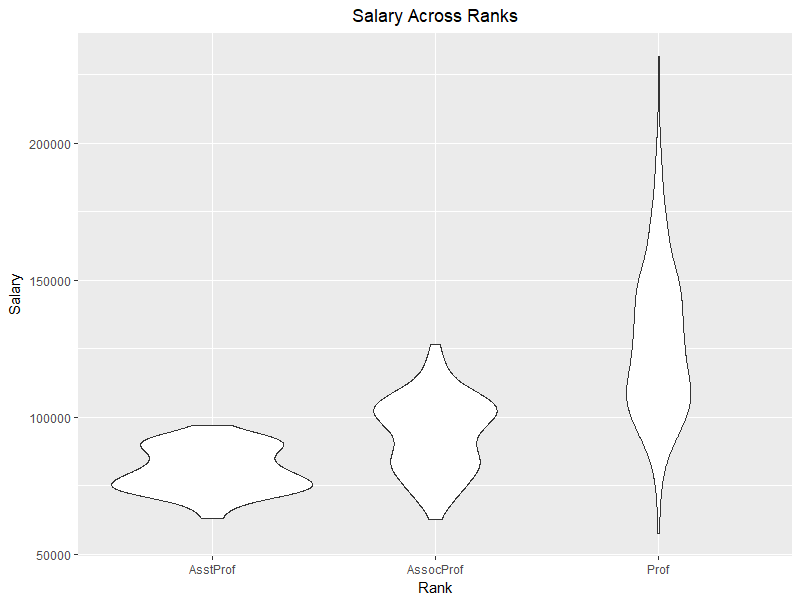
\includegraphics[scale=0.5]{salaryRank}
    \caption{Salary versus Rank}
    \label{pairs3}
\end{figure}

Indeed, in Figure \ref{pairs4} we can see that within each rank, as work experience increases, salaries tend to decrease rather than increase. My hypothesis as to why this is the case, is that highly desirable professors are more likely to have a higher base salary within their rank, and be promoted to the next rank sooner than their less desirable counterparts. In fact, in the full professor rank, there appears to be no relationship between salary and work experience. This could be because once a professor reaches full professorship, his or her value has been established, and incremental changes in work experience have little impact on one's salary. 

\begin{figure}[!htb]
    \centering
    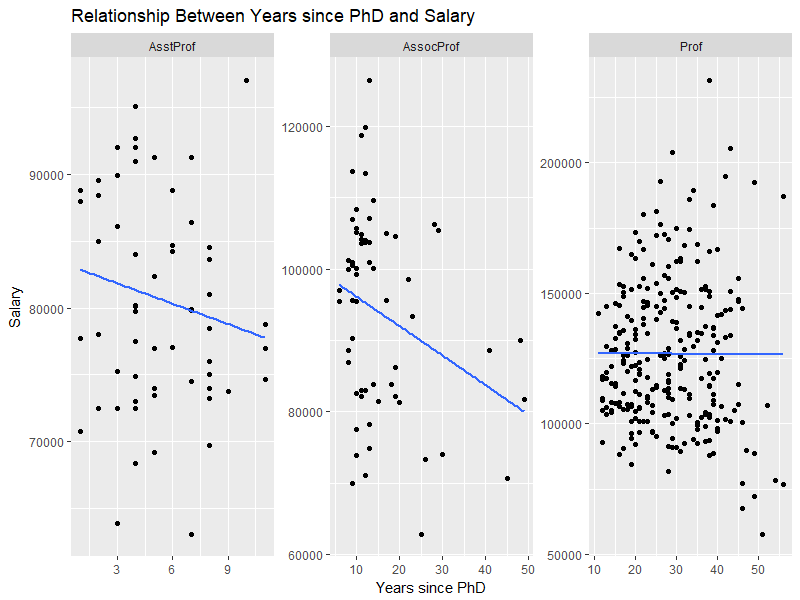
\includegraphics[scale=0.5]{yrsSalary}
    \caption{Salary versus Rank}
    \label{pairs4}
\end{figure}

The applied discipline appears to have a slightly more right skewed distribution than its theoretical counterpart. These relationships are observed in Figure \ref{pairs5}. This could be because of a few influential observations. For instance, certain fields like statistics and computer science are heavily desired by industry, so professors in those fields could demand a higher salary. To reiterate an earlier point: it does not seem to be particularly useful to include discipline as a variable, since the difference in pay across the fields is small, and further, it seems much more relevant to compare professor salaries within particular subject matter, or at the very least to compare across similar subject matter. Like math and physics professors would probably earn similar salaries, but the difference between the salary of a linguist and a computer scientist might be much larger, since the relevant industries pay very different amounts for the respective workers. 

\begin{figure}[!htb]
    \centering
    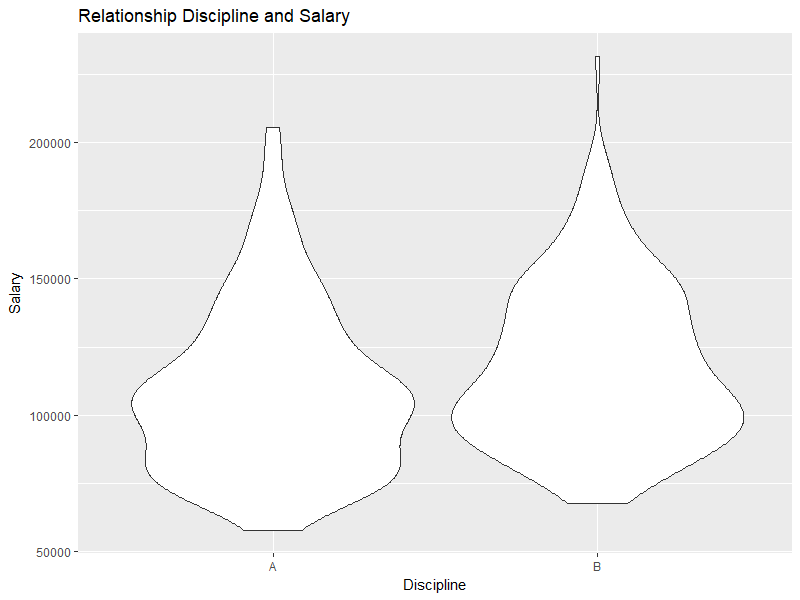
\includegraphics[scale=0.4]{salaryDiscipline}
    \caption{Salary versus Rank}
    \label{pairs5}
\end{figure}

\newpage



\begin{table}[!htb]
\centering
\captionof{table}{Correlations Between Variables} \label{t6} 
\begin{tabular}{rrrr}
  \hline
 & yrs.since.phd & yrs.service & salary \\ 
  \hline
yrs.since.phd & 1.00 & 0.91 & 0.42 \\ 
  yrs.service & 0.91 & 1.00 & 0.33 \\ 
  salary & 0.42 & 0.33 & 1.00 \\ 
   \hline
\end{tabular}
\end{table}

Unsurprisingly, "Years since PhD" and "Years of Service" are highly correlated, thus for a linear model this could cause a problem. In fact, when an OLS linear model is calculated, the variance inflation factors find high values for both "Years since PhD" and "Years of Service" (respectively, 2.68 and 2.41). Confirming the suspicion of multicollinearity\footnote{See appendix for code.}. 
\section{Generalized Additive Model}

To construct a training dataset and a test dataset, I randomly select 80\%\footnote{This was done in class, and many machine learning projects have used similar values.} of the data to use in the training data, and store the remaining data as the test dataset. GAM assumes that the conditional mean of the response surface is a linear combination of functions of the predictors\footnote{These functions need not be linear!}. In other words, we can write: 
\begin{equation}
    Y = \alpha + \sum_{j=1}f_j (\textbf{X}_j) + \epsilon
\end{equation}
and minimize the penalized regression sum of squares. GAM is similar to the single-predictor B-splines, but allows for a different value of $\lambda_j$ for each function in the linear combination of functions of predictors. Thus in a GAM model with the salaries data, the relationship between the predictors and the response(salary) is estimated. GAM being a regularized model, means there will be less concerns about multicollinearity like in the linear model. 

In Figure \ref{gam1sum}\footnote{Located in the appendix.} I report my regression statistics after I regress Salary on "Years since PhD" + "Years of Service" + Rank + Sex + Discipline. The two numerical variables, "Years since PhD" and "Years of Service", had an effective number of degrees of freedom of around $4.58$, which was determined by tuning the equivalent of $\lambda_j$ with the generalized cross-validation statistic(GCV). 

I found statistically significant results for both the rank of full professor, and the applied discipline, at the $p=0.01$ level, and for Sex = Male and the associate professor rank at the $p=0.1$ level. Approximately 53.9\% of the variance is explained by the model. However, in performing a Level 2 analysis, it is difficult for me to convey the uncertainty in the estimates, since there is almost certainly bias in the estimated fitted values. Further, the model selection through the GCV statistic also complicates Level 2 statistical inference. The consequences from the model selection due to the backfitting algorithm make statistical inference problematic. As suspected earlier, it is fairly safe to conclude that the error bands are significantly larger when the data is less sparse. The data points for when there is much work experience, or for recently acquired PhDs, might be of little interpretive value. However, outside the areas with little data, at a Level 1 descriptive analysis, we can see that an increase in work experience does correlate with an increase in salary, but the relationship might actually be negative if the professor has worked at the same college for many years. 

\newpage

\begin{figure}
    \centering
    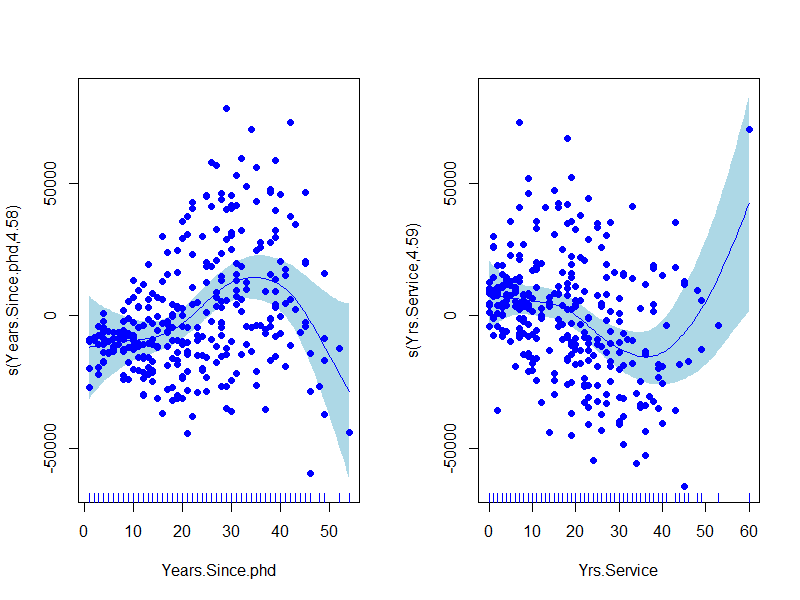
\includegraphics[scale=0.5]{gamPlot}
    \caption{Correlates of the estimated salary for professors at a particular college from the 2008-09 academic year is on each horizontal axis, and the centered fitted values are on each vertical axis, the shaded areas are error bands, with N=317}
    \label{gamplot}
\end{figure}

As mentioned earlier, for points that are at large amounts of work experience, there are larger error values. For points that are not outliers, the model works decently well, as shown in Figure \ref{predict}.

\begin{figure}[!htb]
    \centering
    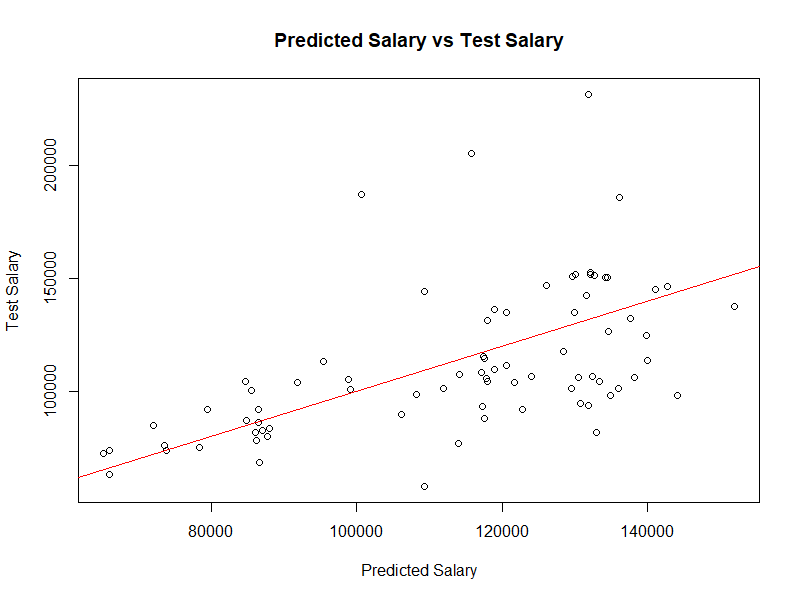
\includegraphics[scale=0.5]{predict}
    \caption{Using the GAM model to predict salary using the test data.}
    \label{predict}
\end{figure}

\newpage

\section{Conclusion}

While there is weak evidence to suggest that female professors are paid less (at the $p=0.1$ level), there is no strong statistical evidence of this. Professor rank appears to be the most critical determinant of salary, and is responsible for the largest differences in salaries between professors. At lower ranks, an increase in service and/or work experience does not correlate positively with an increase in salary, and while I hypothesize why this may be the case, I am not certain about why this is the case. Lastly, discipline does seem to matter. Professors in applied fields tend to make more money than those in theoretical fields. However, as I argue earlier, it might be more relevant to exam professor salaries within subject matter, rather than making the broad distinctions of theoretical versus applied. If there were data on this, it would be interesting to a implement a similar methodology and then examine the results. 


\section{Appendix}

\begin{figure}[!htb]
    \centering
    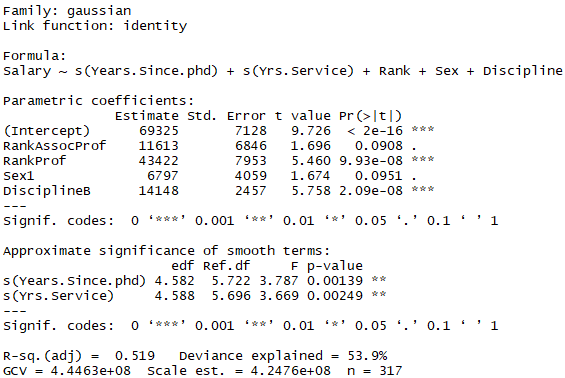
\includegraphics{gam1summary}
    \caption{Summary statistics for basic GAM regression}
    \label{gam1sum}
\end{figure}

\newpage

\begin{verbatim}
library(ggplot2)
library(car)
library(mgcv)
library(xtable)

summary(Salaries)
t1 = table(Salaries$sex, Salaries$rank)

plot1 = ggplot(Salaries, aes(salary))+
  geom_histogram(col="grey", fill ="grey65", binwidth = 5000)+
  theme(plot.title = element_text(hjust = 0.5))+
  labs(title="Salary Histogram")
plot2 = ggplot(Salaries, aes(yrs.service))+
  geom_histogram(col="grey", fill ="grey65", binwidth = 1)+
  theme(plot.title = element_text(hjust = 0.5))+
  labs(title="Years of Service Histogram")
plot3 = ggplot(Salaries, aes(yrs.since.phd))+
  geom_histogram(col="grey", fill ="grey65", binwidth = 1)+
  theme(plot.title = element_text(hjust = 0.5))+
  labs(title="Years since PhD Histogram")

grid.arrange(plot1,plot2,plot3, ncol=2)

plot4 = ggplot(Salaries, aes(yrs.service, fill=sex))+
  geom_histogram(position = "identity", colour ="grey40", binwidth = 1)+
  facet_grid(sex ~ .)+
  labs(title="Years of service for male and female professors")+
  theme(plot.title = element_text(hjust = 0.5))+
  labs(x="Years of Service", y="Count")

plot5 = ggplot(Salaries, aes(yrs.since.phd, fill=sex))+
  geom_histogram(position = "identity", colour ="grey40", binwidth = 1)+
  facet_grid(sex ~ .)+
  labs(title="Years since PhD for male and female professors")+
  theme(plot.title = element_text(hjust = 0.5))+
  labs(x="Years since PhD", y="Count")

grid.arrange(plot4,plot5, ncol=2)


Index<-sample(1:397,80, replace=FALSE)
Test <- Salaries[Index,]
Train <- Salaries[-Index,]

Rank <- Salaries$rank
Discipline <- Salaries$discipline
Years.Since.phd <- Salaries$yrs.since.phd
Yrs.Service <- Salaries$yrs.service
Sex <- as.factor(ifelse(Salaries$sex == "Male",1,0))
sex <- Salaries$sex
Salary <- Salaries$salary
temp <- data.frame(Rank, Discipline, Years.Since.phd, Yrs.Service, Sex, Salary)

tempTrain <- temp[-Index,]
tempTest <- temp[Index,]


out1 <- gam(Salary~s(Years.Since.phd)+s(Yrs.Service)+Rank+Sex+Discipline,data=tempTrain, family=gaussian)
summary(out1)
par(mfrow=c(1,2))
plot(out1, se=T, residuals = T, pch=19, col="blue", shade=T, shade.col = "light blue")


gamPred1 <- predict(out1, newdata = tempTest)
plot(gamPred1, Test$salary, xlab = "Predicted Salary", ylab = "Test Salary", main = "Predicted Salary vs Test Salary")
abline(0,1,col="red")
\end{verbatim}

\end{document}
